\documentclass[aspectratio=169]{beamer}

% Theme and colors
\usetheme{Madrid}
\usecolortheme{default}
\definecolor{rctcblue}{RGB}{0, 51, 102}
\definecolor{rctcgold}{RGB}{255, 204, 0}
\definecolor{codegreen}{RGB}{34, 139, 34}
\setbeamercolor{palette primary}{bg=rctcblue,fg=white}
\setbeamercolor{palette secondary}{bg=rctcblue!80,fg=white}
\setbeamercolor{palette tertiary}{bg=rctcblue!60,fg=white}
\setbeamercolor{structure}{fg=rctcblue}
\setbeamercolor{block title}{bg=rctcblue,fg=white}
\setbeamercolor{block body}{bg=rctcblue!10}
\setbeamercolor{block title alerted}{bg=red!70,fg=white}
\setbeamercolor{block body alerted}{bg=red!10}
\setbeamercolor{block title example}{bg=codegreen,fg=white}
\setbeamercolor{block body example}{bg=codegreen!10}

% Packages
\usepackage{tikz}
\usetikzlibrary{shapes.geometric, arrows.meta, positioning, calc, fit, backgrounds}
% Icons via text (fontawesome5 not available in all distributions)
\usepackage{listings}
\usepackage{booktabs}
\usepackage{graphicx}
\usepackage{hyperref}

% Code listing style
\lstset{
    basicstyle=\ttfamily\small,
    keywordstyle=\color{rctcblue}\bfseries,
    commentstyle=\color{codegreen}\itshape,
    stringstyle=\color{red!70},
    showstringspaces=false,
    breaklines=true,
    frame=single,
    rulecolor=\color{rctcblue!30},
    backgroundcolor=\color{gray!5}
}

% TikZ styles for diagrams
\tikzset{
    llmbox/.style={rectangle, rounded corners, draw=rctcblue, fill=rctcblue!20, 
                   text width=2.5cm, minimum height=1cm, align=center, font=\small},
    agentbox/.style={rectangle, rounded corners, draw=codegreen, fill=codegreen!20,
                     text width=2.5cm, minimum height=1cm, align=center, font=\small},
    toolbox/.style={rectangle, rounded corners, draw=rctcgold!80!black, fill=rctcgold!30,
                    text width=2cm, minimum height=0.8cm, align=center, font=\footnotesize},
    arrow/.style={-{Stealth[length=2mm]}, thick, rctcblue},
    looparrow/.style={-{Stealth[length=2mm]}, thick, codegreen},
}

% Title information
\title[Vibe Coding]{Vibe Coding}
\subtitle{A Guide to Using Agentic AI in Software Development}
\author[B. Shea]{Brendan Shea, PhD}
\institute[RCTC]{Rochester Community and Technical College}
\date{\today}

% Logo (optional - comment out if no logo file)
% \logo{\includegraphics[height=0.8cm]{rctc_logo.png}}

\begin{document}

% ============================================
% SLIDE 1: Title Slide
% ============================================
\begin{frame}
    \titlepage
    \begin{center}
        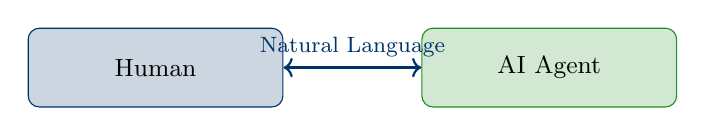
\begin{tikzpicture}
            \node[llmbox, text width=3cm] (human) at (0,0) {Human};
            \node[agentbox, text width=3cm] (ai) at (5,0) {AI Agent};
            \draw[arrow, <->] (human) -- (ai) node[midway, above, font=\footnotesize] {Natural Language};
        \end{tikzpicture}
    \end{center}
\end{frame}

% ============================================
% SLIDE 2: What is Vibe Coding?
% ============================================
\begin{frame}{What is Vibe Coding?}
    \begin{itemize}
        \item \textbf{Vibe coding} is an AI-assisted software development technique where you describe what you want in plain English, and AI generates the code for you.
        \item The term was coined by Andrej Karpathy, co-founder of OpenAI, in February 2025 and quickly became widespread in the developer community.
        \item Collins Dictionary named ``vibe coding'' its Word of the Year for 2025, reflecting how rapidly this approach has entered mainstream technology culture.
        \item Karpathy summarizes the approach simply: ``See things, say things, run things''---you observe a problem, describe it naturally, and execute what the AI produces.
    \end{itemize}
    
    \begin{alertblock}{Key Shift}
        Traditional coding requires you to learn the computer's language (Java, Python, etc.). Vibe coding inverts this: the computer learns to understand \emph{your} language.
    \end{alertblock}
\end{frame}

% ============================================
% SLIDE 3: Why This Matters
% ============================================
\begin{frame}{Why This Matters}
    \begin{itemize}
        \item According to GitLab's 2025 research, 78\% of professional development teams now use AI-assisted coding tools as part of their regular workflow.
        \item This is likely how you will work in your future career---understanding these tools now gives you a significant advantage in the job market.
        \item Here's the key insight: knowing Java (or any programming language) makes you \emph{better} at vibe coding, not obsolete.
        \item Your role shifts from ``person who types code'' to architect, director, and quality inspector---you guide the AI and verify its work.
    \end{itemize}
    
    \begin{block}{Today's Goals}
        \begin{enumerate}
            \item Understand how LLMs and AI agents actually work
            \item Learn the process for building software with AI assistance
            \item Design and prototype your own Swing application
        \end{enumerate}
    \end{block}
\end{frame}

% ============================================
% SLIDE 4: What is a Large Language Model?
% ============================================
\begin{frame}{What is a Large Language Model?}
    \begin{itemize}
        \item A \textbf{Large Language Model (LLM)} is a program trained to predict ``what comes next'' in a sequence of text, based on patterns learned from massive datasets.
        \item LLMs are trained on enormous amounts of text---books, websites, documentation, and millions of lines of source code from public repositories.
        \item Popular examples include GPT (OpenAI), Claude (Anthropic), Gemini (Google), and Llama (Meta), each with different strengths and capabilities.
        \item Critical insight: LLMs don't truly ``know'' things or ``understand'' meaning---they predict statistically likely continuations based on patterns they've seen.
    \end{itemize}
    
    \begin{center}
        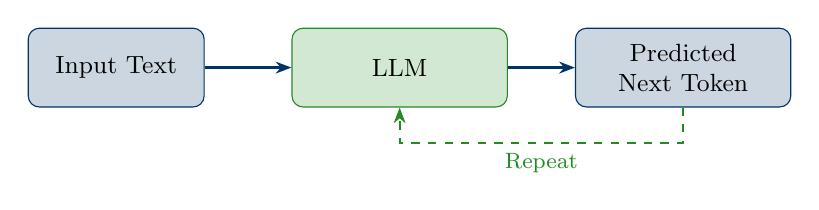
\begin{tikzpicture}[scale=0.9]
            \node[llmbox, text width=2cm] (input) at (0,0) {Input Text};
            \node[agentbox, text width=2.5cm] (llm) at (4,0) {LLM};
            \node[llmbox, text width=2.5cm] (output) at (8,0) {Predicted Next Token};
            \draw[arrow] (input) -- (llm) node[midway, above, font=\footnotesize] {};
            \draw[arrow] (llm) -- (output) node[midway, above, font=\footnotesize] {};
            \draw[looparrow, dashed] (output.south) -- ++(0,-0.5) -| (llm.south) node[pos=0.25, below, font=\footnotesize] {Repeat};
        \end{tikzpicture}
    \end{center}
\end{frame}

% ============================================
% SLIDE 5: Exercise 1 — Seeing Prediction in Action
% ============================================
\begin{frame}{Exercise 1: Seeing Prediction in Action}
    \begin{itemize}
        \item This exercise demonstrates how LLMs work by generating multiple completions for the same starting text.
        \item You'll see that each completion is plausible but different---the model is predicting likely continuations, not retrieving a ``correct'' answer.
        \item Code completions tend to be more predictable than English sentences because programming follows stricter patterns and conventions.
    \end{itemize}
    
    \begin{exampleblock}{Try This (Using Any LLM)}
        \begin{enumerate}
            \item Send: \texttt{Complete this sentence five different ways: "The programmer opened the IDE and"}
            \item Notice how each completion is plausible but different.
            \item Now try: \texttt{Complete this Java code five different ways: "public static void main(String[] args) \{}
            \item \textbf{Reflect}: Why are code completions more predictable than English sentences?
        \end{enumerate}
    \end{exampleblock}
\end{frame}

% ============================================
% SLIDE 6: Tokens — How LLMs Read Text
% ============================================
\begin{frame}{Tokens: How LLMs Read Text}
    \begin{itemize}
        \item A \textbf{token} is the basic unit that LLMs process---roughly 4 characters or about three-quarters of an average English word.
        \item LLMs don't see individual letters or whole words; instead, they break text into these token chunks before processing.
        \item Code gets tokenized too: a method call like \texttt{System.out.println} might become several separate tokens.
        \item Understanding tokens matters because LLMs have a maximum number of tokens they can process at once---this is called the \textbf{context window}.
    \end{itemize}
    
    \begin{center}
        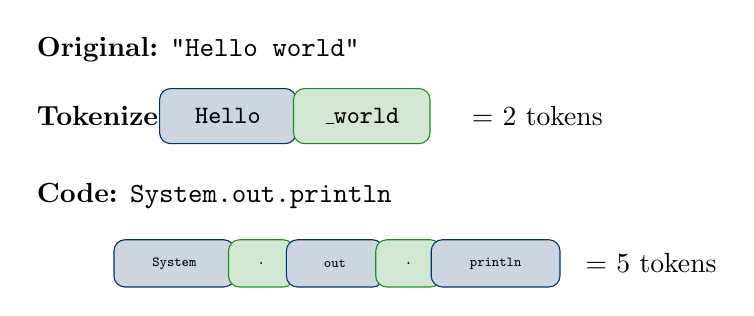
\begin{tikzpicture}[scale=0.85]
            % Original text
            \node[anchor=west] at (0, 1.5) {\textbf{Original:} \texttt{"Hello world"}};
            
            % Tokenized version
            \node[anchor=west] at (0, 0.5) {\textbf{Tokenized:}};
            \node[llmbox, text width=1.5cm, minimum height=0.7cm] at (3, 0.5) {\texttt{Hello}};
            \node[agentbox, text width=1.5cm, minimum height=0.7cm] at (5, 0.5) {\texttt{\_world}};
            \node[anchor=west] at (6.5, 0.5) {= 2 tokens};
            
            % Code example
            \node[anchor=west] at (0, -0.7) {\textbf{Code:} \texttt{System.out.println}};
            \node[llmbox, text width=1.3cm, minimum height=0.6cm, font=\tiny] at (2.2, -1.7) {\texttt{System}};
            \node[agentbox, text width=0.6cm, minimum height=0.6cm, font=\tiny] at (3.5, -1.7) {\texttt{.}};
            \node[llmbox, text width=1cm, minimum height=0.6cm, font=\tiny] at (4.6, -1.7) {\texttt{out}};
            \node[agentbox, text width=0.6cm, minimum height=0.6cm, font=\tiny] at (5.7, -1.7) {\texttt{.}};
            \node[llmbox, text width=1.4cm, minimum height=0.6cm, font=\tiny] at (7, -1.7) {\texttt{println}};
            \node[anchor=west] at (8.2, -1.7) {= 5 tokens};
        \end{tikzpicture}
    \end{center}
\end{frame}

% ============================================
% SLIDE 7: The Context Window
% ============================================
\begin{frame}{The Context Window}
    \begin{itemize}
        \item The \textbf{context window} is the LLM's ``working memory''---the total amount of text it can see and consider at one time during a conversation.
        \item Modern LLMs have large context windows from around 128K tokens (roughly 300 pages) to 1 million tokens or more.
        \item Everything counts toward this limit: your prompt, the conversation history, any code files you share, and the model's own responses.
        \item Once the context window fills up, older content gets pushed out and effectively ``forgotten''---this is why breaking large projects into pieces matters.
    \end{itemize}
    
    \begin{center}
        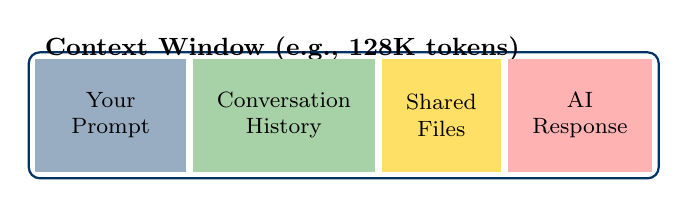
\begin{tikzpicture}[scale=0.8]
            % Context window box
            \draw[thick, rctcblue, rounded corners] (0,0) rectangle (10, 2);
            \node[anchor=north west, font=\small\bfseries] at (0.1, 2.4) {Context Window (e.g., 128K tokens)};
            
            % Segments
            \fill[rctcblue!40] (0.1, 0.1) rectangle (2.5, 1.9);
            \node[font=\footnotesize, align=center] at (1.3, 1) {Your\\Prompt};
            
            \fill[codegreen!40] (2.6, 0.1) rectangle (5.5, 1.9);
            \node[font=\footnotesize, align=center] at (4.05, 1) {Conversation\\History};
            
            \fill[rctcgold!60] (5.6, 0.1) rectangle (7.5, 1.9);
            \node[font=\footnotesize, align=center] at (6.55, 1) {Shared\\Files};
            
            \fill[red!30] (7.6, 0.1) rectangle (9.9, 1.9);
            \node[font=\footnotesize, align=center] at (8.75, 1) {AI\\Response};
        \end{tikzpicture}
    \end{center}
\end{frame}

% ============================================
% SLIDE 8: Exercise 2 — Exploring the Limits
% ============================================
\begin{frame}{Exercise 2: Exploring Context Window Limits}
    \begin{itemize}
        \item This exercise demonstrates that LLM ``memory'' exists only within a single conversation---it cannot remember anything from previous sessions.
        \item Each new conversation starts with a completely blank slate; the model has no knowledge of who you are or what you've discussed before.
        \item This limitation has important implications for large coding projects: you must provide relevant context each time you start a new session.
    \end{itemize}
    
    \begin{exampleblock}{Try This (Using Any LLM)}
        \begin{enumerate}
            \item Start a \textbf{new conversation}. Ask: \texttt{What is my favorite color?}
            \item The LLM doesn't know---it has no context about you.
            \item Now say: \texttt{My favorite color is blue. What is my favorite color?}
            \item It remembers within this conversation!
            \item Start a \textbf{brand new conversation} and ask: \texttt{What is my favorite color?}
            \item \textbf{Reflect}: What does this tell you about working on a project across multiple sessions?
        \end{enumerate}
    \end{exampleblock}
\end{frame}

% ============================================
% SLIDE 9: Why LLMs Are Good at Code
% ============================================
\begin{frame}{Why LLMs Are Good at Code}
    \begin{itemize}
        \item LLMs were trained on millions of public code repositories, so they have ``seen'' countless examples of Java programs, Swing applications, and common coding patterns.
        \item Code is highly structured and predictable---programming languages have strict syntax rules, and developers tend to solve similar problems in similar ways.
        \item Common patterns appear repeatedly across codebases: loops, conditionals, class structures, and standard library calls are all highly predictable sequences.
        \item Key limitation: LLMs can reproduce patterns effectively, but they don't truly ``understand'' program logic or verify that code actually works correctly.
    \end{itemize}
    
    \begin{block}{What This Means for You}
        The LLM has seen thousands of \texttt{JFrame} setups, \texttt{ActionListener} implementations, and \texttt{ArrayList} operations. It can reproduce these patterns fluently---but \emph{you} must verify the logic is correct for your specific needs.
    \end{block}
\end{frame}

% ============================================
% SLIDE 10: Exercise 3 — Testing the Limits
% ============================================
\begin{frame}{Exercise 3: Testing the Limits of ``Understanding''}
    \begin{itemize}
        \item This exercise reveals that LLMs handle common patterns well but struggle with novel or complex logic that requires genuine reasoning.
        \item The first task (checking if a number is even) is a pattern the LLM has seen thousands of times and will likely get correct.
        \item The second task requires combining date logic, calendar rules, and conditional checks---a much less common pattern that often produces buggy code.
    \end{itemize}
    
    \begin{exampleblock}{Try This (Using Any LLM)}
        \scriptsize
        \begin{enumerate}
            \item Ask: \texttt{Write a Java method that returns true if a number is even, false otherwise.}
            \item It will likely get this right (very common pattern).
            \item Now ask: \texttt{Write a Java method that returns true if today is the third Tuesday of the month, but NOT the 12th Tuesday of the year.}
            \item \textbf{Carefully review}: Does this code actually work? Test edge cases!
            \item \textbf{Reflect}: Why was the second task harder? When should you be skeptical of AI-generated code?
        \end{enumerate}
    \end{exampleblock}
\end{frame}

% ============================================
% SLIDE 11: From Chatbot to Agent
% ============================================
\begin{frame}{From Chatbot to Agent}
    \begin{itemize}
        \item A basic LLM is like a conversation partner: you ask a question, it generates a response, and the interaction ends there.
        \item An \textbf{AI agent} combines an LLM with tools and a control loop, allowing it to take actions, observe results, and keep working toward a goal.
        \item The key difference is autonomy: agents can execute multi-step plans, recover from errors, and iterate until a task is complete.
        \item Analogy: asking an LLM for directions gives you a static answer; an agent is like GPS that actively reroutes when you miss a turn.
    \end{itemize}
    
    \begin{center}
        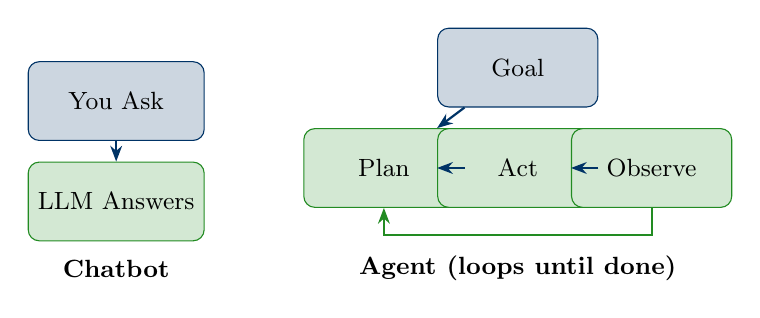
\begin{tikzpicture}[scale=0.85]
            % Chatbot side
            \node[llmbox, text width=2cm] (user1) at (0, 1) {You Ask};
            \node[agentbox, text width=2cm] (llm1) at (0, -0.5) {LLM Answers};
            \draw[arrow] (user1) -- (llm1);
            \node[font=\small\bfseries] at (0, -1.5) {Chatbot};
            
            % Agent side
            \node[llmbox, text width=1.8cm] (goal) at (6, 1.5) {Goal};
            \node[agentbox, text width=1.8cm] (plan) at (4, 0) {Plan};
            \node[agentbox, text width=1.8cm] (act) at (6, 0) {Act};
            \node[agentbox, text width=1.8cm] (observe) at (8, 0) {Observe};
            \draw[arrow] (goal) -- (plan);
            \draw[arrow] (plan) -- (act);
            \draw[arrow] (act) -- (observe);
            \draw[looparrow] (observe.south) -- ++(0, -0.4) -| (plan.south);
            \node[font=\small\bfseries] at (6, -1.5) {Agent (loops until done)};
        \end{tikzpicture}
    \end{center}
\end{frame}

% ============================================
% SLIDE 12: The Agent Loop
% ============================================
\begin{frame}{The Agent Loop}
    \begin{itemize}
        \item AI agents follow a repeated cycle: receive a goal, make a plan, take action, observe the results, and decide what to do next.
        \item This loop continues until the agent determines the goal is achieved, encounters an unrecoverable error, or you manually stop it.
        \item The ``observe'' step is critical: agents can detect compilation errors, test failures, or unexpected output and attempt to fix problems automatically.
        \item This is what makes agent-based coding powerful---but also why human oversight remains essential.
    \end{itemize}
    
    \begin{center}
        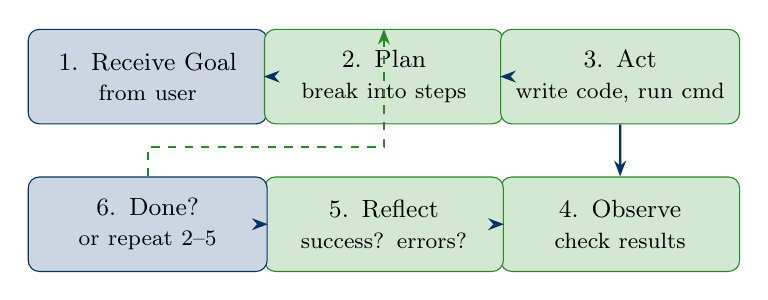
\begin{tikzpicture}[scale=0.75]
            \node[llmbox, text width=2.8cm, minimum height=1.2cm] (receive) at (0, 2) {1. Receive Goal\\{\footnotesize from user}};
            \node[agentbox, text width=2.8cm, minimum height=1.2cm] (plan) at (4, 2) {2. Plan\\{\footnotesize break into steps}};
            \node[agentbox, text width=2.8cm, minimum height=1.2cm] (act) at (8, 2) {3. Act\\{\footnotesize write code, run cmd}};
            \node[agentbox, text width=2.8cm, minimum height=1.2cm] (observe) at (8, -0.5) {4. Observe\\{\footnotesize check results}};
            \node[agentbox, text width=2.8cm, minimum height=1.2cm] (reflect) at (4, -0.5) {5. Reflect\\{\footnotesize success? errors?}};
            \node[llmbox, text width=2.8cm, minimum height=1.2cm] (done) at (0, -0.5) {6. Done?\\{\footnotesize or repeat 2--5}};
            
            \draw[arrow] (receive) -- (plan);
            \draw[arrow] (plan) -- (act);
            \draw[arrow] (act) -- (observe);
            \draw[arrow] (observe) -- (reflect);
            \draw[arrow] (reflect) -- (done);
            \draw[looparrow, dashed] (done.north) -- ++(0, 0.5) -| (plan.north);
        \end{tikzpicture}
    \end{center}
\end{frame}

% ============================================
% SLIDE 13: Tools — Giving the LLM Hands
% ============================================
\begin{frame}{Tools: Giving the LLM Hands}
    \begin{itemize}
        \item On their own, LLMs can only generate text---they cannot actually execute code, create files, or interact with your computer in any way.
        \item \textbf{Tools} are capabilities that let an agent take real actions: reading files, writing code, running terminal commands, compiling programs, and more.
        \item The agent's LLM decides \emph{which} tool to use and \emph{when} based on the current goal and what it observes after each action.
        \item This is what transforms a passive text generator into an active coding assistant that can actually build and test software.
    \end{itemize}
    
    \begin{center}
        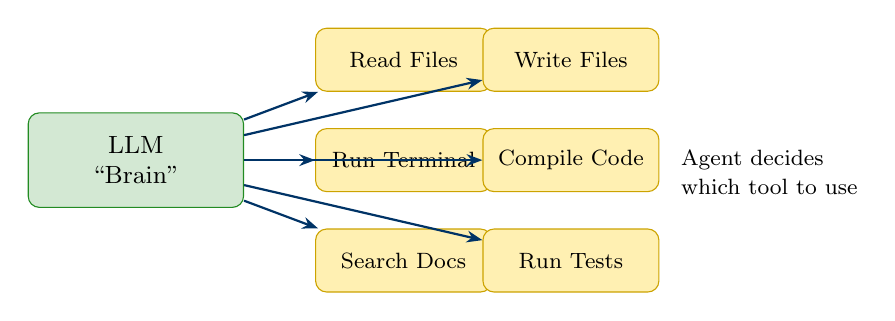
\begin{tikzpicture}[scale=0.85]
            \node[agentbox, text width=2.5cm, minimum height=1.2cm] (llm) at (0, 0) {LLM\\``Brain''};
            
            \node[toolbox] (read) at (4, 1.5) {Read Files};
            \node[toolbox] (write) at (6.5, 1.5) {Write Files};
            \node[toolbox] (terminal) at (4, 0) {Run Terminal};
            \node[toolbox] (compile) at (6.5, 0) {Compile Code};
            \node[toolbox] (search) at (4, -1.5) {Search Docs};
            \node[toolbox] (test) at (6.5, -1.5) {Run Tests};
            
            \draw[arrow] (llm) -- (read);
            \draw[arrow] (llm) -- (write);
            \draw[arrow] (llm) -- (terminal);
            \draw[arrow] (llm) -- (compile);
            \draw[arrow] (llm) -- (search);
            \draw[arrow] (llm) -- (test);
            
            \node[font=\footnotesize, anchor=west] at (8, 0) {Agent decides};
            \node[font=\footnotesize, anchor=west] at (8, -0.4) {which tool to use};
        \end{tikzpicture}
    \end{center}
\end{frame}

% ============================================
% SLIDE 14: Exercise 4 — Thinking Like an Agent
% ============================================
\begin{frame}{Exercise 4: Thinking Like an Agent}
    \begin{itemize}
        \item This exercise helps you understand how agents break down tasks into steps and anticipate what could go wrong at each stage.
        \item By asking the LLM to \emph{plan} rather than \emph{code}, you learn to think at the architectural level---a crucial skill for directing AI effectively.
        \item Understanding the agent's decision-making process helps you write better prompts and catch problems before they compound.
    \end{itemize}
    
    \begin{exampleblock}{Try This (Using Any LLM)}
        \scriptsize
        \begin{enumerate}
            \item Ask: \texttt{If you were an AI agent with tools to read files, write files, and run terminal commands, describe step-by-step how you would add a "Save" button to an existing Java Swing app. Don't write code---just describe your plan.}
            \item Read the plan carefully. Does it make sense?
            \item Now ask: \texttt{What could go wrong at each step? How would you detect and fix each problem?}
            \item \textbf{Reflect}: How is asking for a \emph{plan} different from asking the agent to ``just do it''?
        \end{enumerate}
    \end{exampleblock}
\end{frame}

% ============================================
% SLIDE 15: Why Agents Still Need You
% ============================================
\begin{frame}{Why Agents Still Need You}
    \begin{itemize}
        \item Agents optimize for ``looks complete'' rather than ``actually correct''---they may produce code that compiles but contains subtle logic errors.
        \item The agent only knows what you tell it; it cannot read your mind about unstated requirements, edge cases, or how the software should ``feel'' to users.
        \item Agents can get stuck in loops, make things worse while trying to fix errors, or confidently produce insecure or inefficient code.
        \item Your role is essential: you are the \textbf{architect} who designs the system, the \textbf{director} who guides the work, and the \textbf{inspector} who verifies quality.
    \end{itemize}
    
    \begin{alertblock}{The Human-Agent Partnership}
        \begin{tabular}{ll}
            \textbf{Agent's Job:} & Generate code, run commands, iterate on errors \\
            \textbf{Your Job:} & Define requirements, design architecture, verify correctness \\
        \end{tabular}
    \end{alertblock}
\end{frame}

% ============================================
% SLIDE 16: Setup & Tools Overview
% ============================================
\begin{frame}{Setup \& Tools Overview}
    \begin{itemize}
        \item To use AI coding agents, you need an account with an AI provider (like GitHub Copilot, which is free for students) and an editor that supports agent mode.
        \item The specific tools and interfaces change rapidly---detailed setup instructions are on the course website and will be updated as needed.
        \item What matters most is understanding the \emph{concepts}: once you understand how agents work, you can adapt to any specific tool.
    \end{itemize}
    
    \begin{block}{Key Components (Tools May Vary)}
        \begin{enumerate}
            \item \textbf{AI Provider Account}: GitHub Copilot (free via Student Developer Pack), Claude, ChatGPT, or others
            \item \textbf{Code Editor}: VS Code, IntelliJ, or other IDE with AI integration
            \item \textbf{Agent Mode}: The autonomous mode where AI can read/write files and run commands
            \item \textbf{Chat Mode}: For asking questions, getting explanations, and requesting snippets
        \end{enumerate}
    \end{block}
\end{frame}

% ============================================
% SLIDE 17: The Vibe Coding Paradox
% ============================================
\begin{frame}{The Vibe Coding Paradox}
    \begin{itemize}
        \item AI makes generating code dramatically faster---what once took hours can now take minutes, and what took days can take hours.
        \item However, this speed also makes generating \emph{bad} code faster; without discipline, you can create a tangled mess in record time.
        \item The \textbf{vibe coding paradox}: the easier it becomes to generate code, the more important process and planning become.
        \item Speed without direction means you get lost faster---you need a clear destination before you start moving quickly.
    \end{itemize}
    
    \begin{alertblock}{The Core Tension}
        \centering
        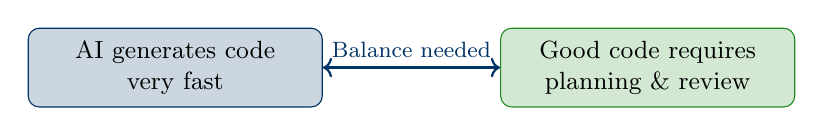
\begin{tikzpicture}
            \node[llmbox, text width=3.5cm] (fast) at (0, 0) {AI generates code\\very fast};
            \node[agentbox, text width=3.5cm] (good) at (6, 0) {Good code requires\\planning \& review};
            \draw[arrow, <->] (fast) -- (good) node[midway, above, font=\footnotesize] {Balance needed};
        \end{tikzpicture}
    \end{alertblock}
\end{frame}

% ============================================
% SLIDE 18: Exercise 5 — The "Everything at Once" Disaster
% ============================================
\begin{frame}{Exercise 5: The ``Everything at Once'' Disaster}
    \begin{itemize}
        \item This exercise demonstrates why asking for too much at once leads to problematic results---even when the AI appears to succeed.
        \item You'll experience firsthand how difficult it is to understand, debug, and modify code when you didn't build it piece by piece.
        \item The goal is not to discourage ambition, but to show why breaking work into smaller pieces produces better outcomes.
    \end{itemize}
    
    \begin{exampleblock}{Try This (Using Any LLM)}
        \scriptsize
        \begin{enumerate}
            \item Ask: \texttt{Write a complete Java Swing task manager with categories, due dates, priorities, search functionality, and the ability to save/load from a file.}
            \item Examine the result and answer these questions:
            \begin{itemize}
                \item How many lines of code did it generate?
                \item Can you explain what every section does?
                \item Does it actually compile and run correctly?
                \item If there's a bug, where would you start looking?
            \end{itemize}
            \item \textbf{Reflect}: What would have been a smarter \emph{first} prompt?
        \end{enumerate}
    \end{exampleblock}
\end{frame}

% ============================================
% SLIDE 19: The Software Development Lifecycle (SDLC)
% ============================================
\begin{frame}{The Software Development Lifecycle (SDLC)}
    \begin{itemize}
        \item The \textbf{Software Development Lifecycle (SDLC)} is a structured process that professional developers follow to build reliable, maintainable software.
        \item AI accelerates the Implementation phase dramatically, but it cannot replace the other phases---in fact, they become more important.
        \item Skipping Requirements or Design means the AI has no clear target; skipping Testing means bugs slip through; skipping Maintenance planning means future changes become painful.
    \end{itemize}
    
    \begin{center}
        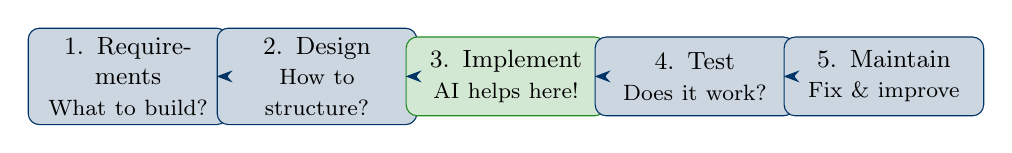
\begin{tikzpicture}[scale=0.8]
            \node[llmbox, text width=2.3cm, minimum height=1cm] (req) at (0, 0) {1. Requirements\\{\footnotesize What to build?}};
            \node[llmbox, text width=2.3cm, minimum height=1cm] (des) at (3, 0) {2. Design\\{\footnotesize How to structure?}};
            \node[agentbox, text width=2.3cm, minimum height=1cm] (imp) at (6, 0) {3. Implement\\{\footnotesize AI helps here!}};
            \node[llmbox, text width=2.3cm, minimum height=1cm] (test) at (9, 0) {4. Test\\{\footnotesize Does it work?}};
            \node[llmbox, text width=2.3cm, minimum height=1cm] (maint) at (12, 0) {5. Maintain\\{\footnotesize Fix \& improve}};
            
            \draw[arrow] (req) -- (des);
            \draw[arrow] (des) -- (imp);
            \draw[arrow] (imp) -- (test);
            \draw[arrow] (test) -- (maint);
        \end{tikzpicture}
    \end{center}
\end{frame}

% ============================================
% SLIDE 20: Incremental Development — The Golden Rule
% ============================================
\begin{frame}{Incremental Development: The Golden Rule}
    \begin{itemize}
        \item \textbf{Incremental development} means building software in small, testable pieces rather than trying to create everything at once.
        \item Each piece should be small enough to understand completely, test thoroughly, and fix easily if something goes wrong.
        \item This approach aligns perfectly with how AI agents work best: focused tasks with clear success criteria produce much better results than vague, sprawling requests.
        \item Professional developers call this ``Agile'' methodology---and it's even more important when working with AI.
    \end{itemize}
    
    \begin{block}{The Incremental Process}
        \scriptsize
        \begin{enumerate}
            \item Build the smallest working piece first (e.g., just a window)
            \item Test it---does it work correctly?
            \item Add the next piece (e.g., a list display)
            \item Test again---does everything still work?
            \item Repeat until the application is complete
        \end{enumerate}
    \end{block}
\end{frame}

% ============================================
% SLIDE 21: Exercise 6 — Breaking Down a Project
% ============================================
\begin{frame}{Exercise 6: Breaking Down a Project}
    \begin{itemize}
        \item This exercise uses the LLM as a planning partner to help you decompose a project into manageable, buildable pieces.
        \item The key skill here is learning to think architecturally: what are the components, and in what order should they be built?
        \item Save the output from this exercise---you will use this breakdown to guide your actual implementation later.
    \end{itemize}
    
    \begin{exampleblock}{Try This (Using Any LLM)}
        \scriptsize
        \begin{enumerate}
            \item Choose a simple app idea (or use: ``a flashcard study app'')
            \item Ask: \texttt{I want to build a [your app] using Java Swing. Help me break this into 5--6 small pieces I could build one at a time. Each piece should be testable on its own. List them in build order.}
            \item Review: Does the order make sense? Would each piece work alone?
            \item Ask: \texttt{For piece \#1, what would I see on screen when it's working?}
            \item \textbf{Save this list}---you'll use it for your project!
        \end{enumerate}
    \end{exampleblock}
\end{frame}

% ============================================
% SLIDE 22: Anatomy of an Effective Prompt
% ============================================
\begin{frame}{Anatomy of an Effective Prompt}
    \begin{itemize}
        \item A \textbf{prompt} is the instruction or request you give to an LLM; the quality of your prompt directly determines the quality of the output.
        \item Effective prompts share four key elements: context about what exists, a specific task, constraints to follow, and guidance on quality.
        \item Think of prompting as giving instructions to a skilled but literal-minded assistant who has no background knowledge about your specific project.
    \end{itemize}
    
    \begin{block}{The Four Elements of a Good Prompt}
        \scriptsize{
        \begin{tabular}{p{2.5cm} p{9cm}}
            \toprule
            \textbf{Element} & \textbf{What to Include} \\
            \midrule
            1. Context & What already exists? What are you building? \\
            2. Specific Task & What exactly should this step accomplish? \\
            3. Constraints & Language, libraries, patterns, limitations \\
            4. Quality Guidance & ``Add comments,'' ``Keep it simple,'' ``Explain first'' \\
            \bottomrule
        \end{tabular}
        }
    \end{block}
\end{frame}

% ============================================
% SLIDE 23: Exercise 7 — Good Prompt vs. Bad Prompt
% ============================================
\begin{frame}{Exercise 7: Good Prompt vs.\ Bad Prompt}
    \begin{itemize}
        \item This exercise lets you directly compare the results of a vague prompt versus a detailed, well-structured prompt.
        \item You'll see how specificity dramatically improves the usefulness and correctness of AI-generated code.
        \item The extra time spent writing a good prompt is recovered many times over by reducing debugging and confusion.
    \end{itemize}
    
    \begin{exampleblock}{Try Both Prompts (Using Any LLM)}
        \scriptsize
        \textbf{Prompt A} (vague): \texttt{Make a Java GUI with a list and buttons.}
        
        \vspace{0.3em}
        \textbf{Prompt B} (specific): \texttt{Create a Java Swing JFrame (500x400 pixels) with BorderLayout. In the center, add a JList displaying String items. At the bottom (SOUTH), add a JPanel with two buttons labeled "Add" and "Remove". No functionality yet---just the layout. Add comments explaining each component.}
        
        \vspace{0.3em}
        Compare the outputs: Which is more useful? More understandable? Try running both---which works better? \textbf{Reflect}: What made Prompt B more effective?
    \end{exampleblock}
\end{frame}

% ============================================
% SLIDE 24: The Iteration Mindset
% ============================================
\begin{frame}{The Iteration Mindset}
    \begin{itemize}
        \item \textbf{Iteration} means repeatedly refining your work through cycles of attempt, feedback, and improvement---this is normal and expected in vibe coding.
        \item Don't expect perfection on the first try; even expert prompters go back and forth with the AI to get the result they want.
        \item When something doesn't work, describe \emph{specifically} what went wrong rather than just saying ``it doesn't work'' or ``try again.''
        \item Treat the interaction like a conversation with a colleague: you guide, it types, you review, you refine together.
    \end{itemize}
    
    \begin{center}
        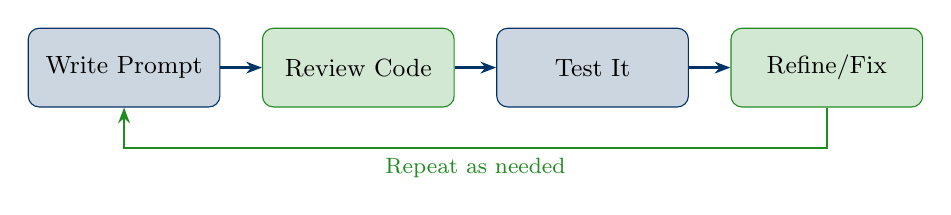
\begin{tikzpicture}[scale=0.85]
            \node[llmbox, text width=2.2cm] (prompt) at (0, 0) {Write Prompt};
            \node[agentbox, text width=2.2cm] (review) at (3.5, 0) {Review Code};
            \node[llmbox, text width=2.2cm] (test) at (7, 0) {Test It};
            \node[agentbox, text width=2.2cm] (refine) at (10.5, 0) {Refine/Fix};
            
            \draw[arrow] (prompt) -- (review);
            \draw[arrow] (review) -- (test);
            \draw[arrow] (test) -- (refine);
            \draw[looparrow] (refine.south) -- ++(0, -0.6) -| (prompt.south) node[pos=0.25, below, font=\footnotesize] {Repeat as needed};
        \end{tikzpicture}
    \end{center}
\end{frame}

% ============================================
% SLIDE 25: Exercise 8 — The Iteration Loop in Practice
% ============================================
\begin{frame}{Exercise 8: The Iteration Loop in Practice}
    \begin{itemize}
        \item This exercise gives you hands-on experience with the iteration loop by building on code from Exercise 7 and adding functionality.
        \item You'll practice the most important vibe coding skill: describing problems specifically when something doesn't work.
        \item Notice how many back-and-forth exchanges it takes---this is completely normal, not a sign of failure.
    \end{itemize}
    
    \begin{exampleblock}{Try This (Continuing from Exercise 7, Prompt B)}
        \begin{enumerate}
            \item Take the GUI code from Prompt B (the JFrame with JList and buttons)
            \item Ask: \texttt{Add an ActionListener to the "Add" button. When clicked, show a JOptionPane input dialog asking for text, then add that text to the JList.}
            \item Test it---does it work? If not, describe the specific problem.
            \item If it works, ask: \texttt{Now make the "Remove" button delete the currently selected item from the list.}
            \item \textbf{Reflect}: How many exchanges did it take? What did you learn?
        \end{enumerate}
    \end{exampleblock}
\end{frame}

% ============================================
% SLIDE 26: Choosing Your Project
% ============================================
\begin{frame}{Choosing Your Project}
    \begin{itemize}
        \item For the remainder of this lecture and your homework, you will design and build your own Java Swing application using AI assistance.
        \item Choose something simple that interests you---enthusiasm helps you push through challenges, and simplicity ensures you can actually finish.
        \item Your app must have a graphical interface with at least three interactive components (buttons, text fields, lists, etc.).
        \item Remember: you can always add more features later; start with a minimal version that actually works.
    \end{itemize}
    
    \begin{block}{Project Ideas (Pick One or Invent Your Own)}
        \begin{tabular}{p{5cm} p{6cm}}
            Task manager / To-do list & Flashcard study app \\
            Simple quiz game & Habit tracker \\
            Recipe organizer & Tip calculator \\
            Unit converter & Countdown timer \\
            Personal diary / journal & Password generator \\
        \end{tabular}
    \end{block}
\end{frame}

% ============================================
% SLIDE 27: Exercise 9 — AI-Assisted Requirements
% ============================================
\begin{frame}{Exercise 9: AI-Assisted Requirements}
    \begin{itemize}
        \item \textbf{Requirements} define what your software should do---they are the foundation that everything else builds upon.
        \item In this exercise, you'll use the LLM as a collaborator to help you think through what features your app needs.
        \item The goal is not to accept everything the AI suggests, but to use its suggestions as a starting point for your own decisions.
    \end{itemize}
    
    \begin{exampleblock}{Try This (Using Any LLM)}
        \scriptsize
        \begin{enumerate}
            \item Decide on your app idea from the previous slide
            \item Ask: \texttt{I'm a beginner building a [your app] in Java Swing. Help me define clear requirements. What are 4--5 core features a simple version should have? Keep it realistic for a beginner.}
            \item Review the suggestions---are they too ambitious? Too simple?
            \item Ask: \texttt{For each feature, what would the user actually DO? (click, type, select, etc.)}
            \item \textbf{Write down your final list of 4--5 features}
        \end{enumerate}
    \end{exampleblock}
\end{frame}

% ============================================
% SLIDE 28: Exercise 10 — AI-Assisted Design
% ============================================
\begin{frame}{Exercise 10: AI-Assisted Design}
    \begin{itemize}
        \item \textbf{Design} determines how your software will be structured---what components exist and how they fit together.
        \item This exercise helps you visualize your application's interface and plan the order in which you'll build each piece.
        \item Creating a sketch (even a rough one on paper) before coding dramatically reduces confusion and wasted effort.
    \end{itemize}
    
    \begin{exampleblock}{Try This (Using Any LLM)}
        \scriptsize
        \begin{enumerate}
            \item Describe your app and features from Exercise 9 to the LLM
            \item Ask: \texttt{Describe what the main window should look like. What Swing components would I need? Where should each go?}
            \item Ask: \texttt{What Java classes or data structures will I need to store the app's data?}
            \item Ask: \texttt{Break this into 5--6 pieces I should build incrementally. What order?}
            \item \textbf{Sketch the window on paper and number your build order}
        \end{enumerate}
    \end{exampleblock}
\end{frame}


% ============================================
% SLIDE 29: Exercise 11 — Start Building Your Project
% ============================================
\begin{frame}{Exercise 11: Start Building Your Project}
    \begin{itemize}
        \item Now it's time to start actually building---using everything you've learned about incremental development and effective prompting.
        \item Begin with piece \#1 from your design (usually the basic window with layout) and don't move on until it works correctly.
        \item Use the prompt pattern: provide context, specify the task clearly, add constraints, and request comments for learning.
    \end{itemize}
    
    \begin{exampleblock}{Start Building (Using Agent Mode or Chat)}
        \scriptsize
        \begin{enumerate}
            \item Create a new project folder for your application
            \item Build \textbf{only piece \#1} from your plan (e.g., basic window with layout)
            \item Suggested prompt pattern: \texttt{Create a Java Swing [component] for a [your app]. [Specific details about size, layout, labels]. Add comments explaining each part. This is step 1---keep it simple.}
            \item \textbf{Test it}: Does the window appear? Does it look right?
            \item If yes: save your work and move to piece \#2
            \item If no: describe the problem specifically and iterate
        \end{enumerate}
    \end{exampleblock}
\end{frame}

% ============================================
% SLIDE 30: Vibe Coding Best Practices
% ============================================
\begin{frame}{Vibe Coding Best Practices}
    \begin{itemize}
        \item These seven practices separate successful vibe coders from those who end up frustrated with tangled, broken code.
        \item Notice that most of these practices happen \emph{before} or \emph{after} the AI generates code---the human work remains essential.
        \item Treat these as habits to build; they will serve you throughout your programming career, with or without AI assistance.
    \end{itemize}
    
    \begin{block}{Seven Habits of Effective Vibe Coders}
        \scriptsize
        \begin{enumerate}
            \item \textbf{Plan before prompting}---know what you're building
            \item \textbf{Build incrementally}---one working piece at a time
            \item \textbf{Review everything}---never accept code you don't understand
            \item \textbf{Test after each change}---catch problems early
            \item \textbf{Ask for explanations}---use AI to learn, not just produce
            \item \textbf{Keep prompts focused}---one task per prompt works best
            \item \textbf{Iterate willingly}---back-and-forth is normal, not failure
        \end{enumerate}
    \end{block}
\end{frame}

% ============================================
% SLIDE 31: Common Pitfalls to Avoid
% ============================================
\begin{frame}{Common Pitfalls to Avoid}
    \begin{itemize}
        \item Learning from others' mistakes is faster than making them all yourself---these are the most common ways vibe coding goes wrong.
        \item Most pitfalls stem from either asking for too much at once or accepting results without sufficient scrutiny.
        \item When you catch yourself falling into one of these traps, pause and return to the fundamentals: plan, build small, test, review.
    \end{itemize}
    
    \begin{alertblock}{Six Ways Vibe Coding Goes Wrong}
        \scriptsize
        \begin{tabular}{p{1cm} p{10.5cm}}
            \textcolor{red!70}{\textbf{1.}} & Dumping huge requirements into a single prompt \\
            \textcolor{red!70}{\textbf{2.}} & Accepting code you don't understand \\
            \textcolor{red!70}{\textbf{3.}} & Skipping testing because ``the AI wrote it'' \\
            \textcolor{red!70}{\textbf{4.}} & Not learning fundamentals (``I'll just ask AI'') \\
            \textcolor{red!70}{\textbf{5.}} & Ignoring security, edge cases, and error handling \\
            \textcolor{red!70}{\textbf{6.}} & Giving up when the first result isn't perfect \\
        \end{tabular}
    \end{alertblock}
\end{frame}

% ============================================
% SLIDE 32: Key Takeaways & Homework
% ============================================
\begin{frame}{Key Takeaways \& Homework}
    \begin{block}{What You Learned Today}
        \begin{itemize}
            \item \textbf{LLMs} predict text based on patterns; \textbf{agents} add tools and loops to accomplish goals autonomously
            \item Process matters more than ever: requirements $\rightarrow$ design $\rightarrow$ incremental build $\rightarrow$ test
            \item Good prompts are specific, contextual, and focused on one piece at a time
            \item Your Java knowledge makes you \emph{better} at vibe coding, not obsolete---you are the architect
        \end{itemize}
    \end{block}
    
    \begin{exampleblock}{Homework Assignment}
        \scriptsize
        \begin{enumerate}
            \item Complete your Swing application (minimum 3 working features)
            \item Submit the following:
            \begin{itemize}
                \item Your requirements list (from Exercise 9)
                \item Your design sketch and build order (from Exercise 10)
                \item Three example prompts you used and what they produced
                \item Your working Java code
            \end{itemize}
            \item Be prepared to demo your app and explain how you built it
        \end{enumerate}
    \end{exampleblock}
\end{frame}


\end{document}